%!TEX root = ../main.tex
\section{Node Software}
\label{sec:node_software}
When addressing the node software it is important to remember the distinction between sensor node software and WiFi node software.
The software for the WiFi node has not been implemented therefore this section will only address the verification of the functionalities of the sensor node software implemented on a GPS sensor node.

\subsection{GPS Sensor Node}
The functionality of the developed GPS sensor node software was tested as shown in figure \ref{fig:sensor_gps_veri}.
The GPS service virtualization was run to input data as a GPS module does. 
The GPS node software then processed the data and output it to standard output as the CAN bus connection was not realized.

\begin{figure}[h]
	\centering
	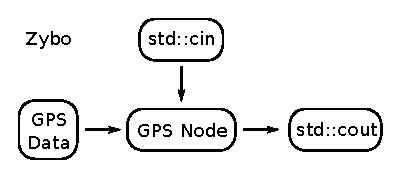
\includegraphics[width = 0.6\linewidth]{graphics/sensor_gps_veri}
	\caption[Testing node software.]{Testing the node software. The node software receives data from a list of GPS data and inputs from \texttt{std::cin}. It outputs to \texttt{std::cout}.}
	\label{fig:sensor_gps_veri}
\end{figure}

When running the software is run it outputs only a string of booleans. 
This is not very readable by humans, so to show the functionality the program was set to print in a humanly understandable way.
A segment of the output from this can be seen in code \ref{code:output_node}.
The first frame should be a timestamp frame.
It can be seen that the the first frame has node ID 14, 4 data bytes, message type 1 and data 2374, meaning that it is from the GPS node with a timestamp of 2374 milliseconds.
The next frame should then be a data frame containing latitude and longitude information.
It can be seen that it has node ID 14, 8 data bytes and message type 9, which is a latitude longitude message.
To extract the latitude and longitude from the data field an unpacking algorithm is needed.
Using that it is found that latitude is 55.3673346 degrees North and longitude is 10.4318456 degrees East.

\begin{lstlisting}[caption=Struct for data packet.,label=code:output_node]
(*@\makebox[\linewidth][c]{$\smash{\vdots}$}@*)
Start of frame: 1
Node id: 1110
Number of data bytes: 0100
Message type: 000001
Data: 00000000000000000000100101000110
Full frame: 11110000001010000000000000000000000100101000110

Start of frame: 1
Node id: 1110
Number of data bytes: 1000
Message type: 001001
Data: 00100001000000000110001010000010000001100011011111000101 11111000
Full frame: 11110001001100000100001000000000110001010000010000 00110001101111100010111111000
(*@\makebox[\linewidth][c]{$\smash{\vdots}$}@*)
\end{lstlisting}

It should be possible to send a sync command to the node by giving it the message ID \texttt{10001111000}.
When typing this into the shell it can be seen that the nodes timestamp is reset.
By sending the message ID \texttt{10001111010} the node stops outputting data.
The node starts sending data again if the message ID \texttt{10001111001} is sent.\\

The link to the CAN program is not made and therefore the tests are made with standard I/O.
By using service virtualization it is verified that the GPS sensor node software has implemented the wanted functionalities.
